\section[Wstęp do api OpenCL]{Wstęp do api OpenCL}
OpenCL (ang. Open Compute Language) to standard tworzony obecnie przez grupę Khronos, służący do pisania programów, które mogą zostać wykonane na różnych platformach takich jak CPU (ang. Centrall Processing Unit), GPU (ang. Graphics Processing Unit) czy FPGA (ang. Field-Programmable Gate Array). Specyfikacja OpenCL definiuje interfejs w języku C++, który umożliwia zaprogramowanie aplikacji, by ta wykonała konkretny kod na wybranym urządzeniu. Standard OpenCL jest głównie wykorzystywany do równoległych obliczeń, takich jak wektorowe operacje matematyczne czy przetwarzanie obrazów. Za implementacje sterownika, który wystawia api, zgodne z określoną wersją specyfikacji, odpowiedzialny jest producent urządzenia.  Dzięki temu, że standard jest otwarty, a jego implementacje posiada większość producentów, możliwe jest stworzenie kodu, który można uruchomić niezależnie od architektury czy producenta posiadanego procesora głównego czy graficznego. Jest to duża zaleta w porównaniu na przykład do CUDA, która to jest interfejsem implementowanym jedynie przez NVidie. Standard OpenCL jest rozwijany i modyfikowany, przez co api zdefiniowane jest w kilku wersjach. Najnowsza wersja specyfikacji to wersja 3.0. Wszystkie wersje są kompatybilne wstecznie. Dodatkowo zdefiniowane są rozszerzenia api, takie jak cl\_khr\_gl\_sharing, czyli definiujące api do współdzielenia (tzw. sharingu) obiektów między OpenCL a OpenGL. Takie dodatkowe api jest też specyfikowane przez grupę Khonosa w ramach określonej wersji OpenCL, jednak nie jest obowiązkowe. Istnieją także rozszerzenia api wyspecyfikowane przez konkretnego producenta, np. cl\_intel\_mem\_force\_host\_memory, które jest dostępna na urządzeniach intela lub cl\_qcom\_android\_native\_buffer\_host\_ptr dostępny na procesorach Qualcoma z systemem Android. Takie dodatkowe api uzupełnia podstawę, umożliwiając lepsze dopasowanie specyfikacji do konkretnego sprzętu. OpenCL na platformie Android dostępny jest jedynie z poziomu natywnej biblioteki w języku C++. Na urządzeniach z systemem macOS środowisko te nie jest wspierane.

\subsection{Linkowanie biblioteki OpenCL na platformie Android}
Aplikacje zwykle nie linkują się bezpośrednio ze sterownikiem posiadającym kompletną implementację api. Do tego wykorzystywana jest dodatkowa biblioteka, która wyszukuje implementacji sterownika dla wszystkich platform na urządzeniu. Dzięki wykorzystaniu takiej ładującej biblioteki aplikacja może używać każdej dostępnej platformy wspierającej to api oraz nie jest na sztywno połączona z jednym sterownikiem w określonej wersji.
Niestety binarna wersja takiej biblioteki dla systemu Android nie istnieje. Jedną z możliwości jest połączenie natywnej biblioteki ze sterownikiem znajdującym się w urządzeniu. Wadą takiego rozwiązania jest konieczność pobrania z urządzenia pliku binarnego z implementacją OpenCL oraz wszystkich zależnych od niej sterowników. Takie rozwiązanie powoduje, że skompilowana aplikacja będzie działać jedynie na urządzeniu, z którego zostały pobrane biblioteki.
Innym rozwiązaniem jest pobranie źródeł z kodem biblioteki ładującej, zbudowanie biblioteki i połączenie jej z aplikacją. Sterownik, który będzie łączył program z implementacją OpenCL, ma zapisane domyślne ścieżki, w których mogą znajdować sie biblioteka OpenCL. Istnieje również możliwość zdefiniowania zmiennej środowiskowej, posiadającej lokalizację z której chcemy by sterownik został załadowany. Wadą takiego rozwiązania jest konieczność kompilacji takiej biblioteki, natomiast dzięki temu możemy zbudować aplikację działającą na wielu urządzeniach.
\begin{figure}[H]
	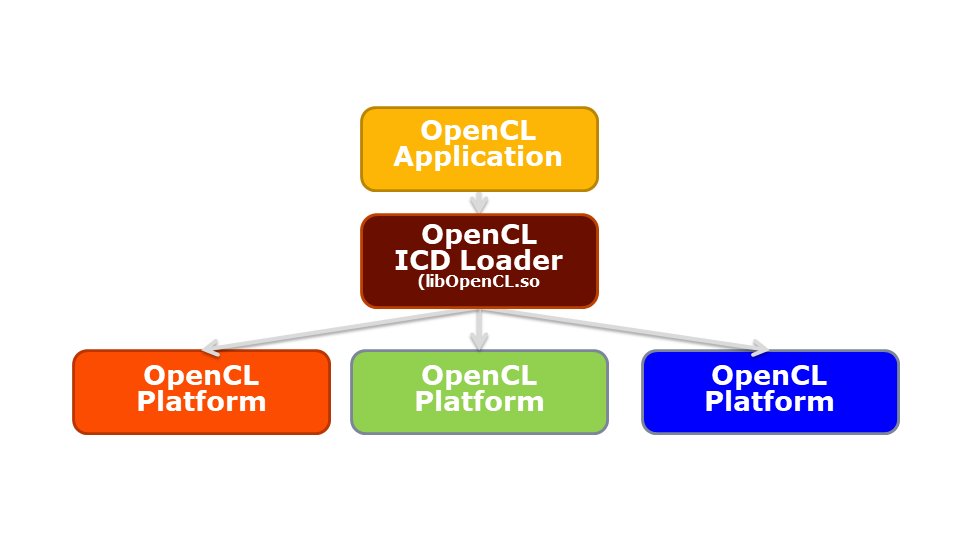
\includegraphics[scale=0.4]{imgs/icdLoader.png}
	\caption{Linkowanie biblioteki OpenCL \cite{Loader}}
\end{figure}
Powyższy obrazek ilustruje w jaki sposób aplikacje łączą się z implementacją sterownika dla konkretnego urządzenia. Aplikacja może odpytać każde urządzenie o jego właściwości, a następnie wybrać te na którym uruchomi się dalsza część aplikacji.

\subsection{Typowy przebieg aplikacji OpenCL}
Poniżej widać jak wygląda przebieg prostego programu wykoystującego api OpenCL do inkrementowania każdego elementu bufora pamięci.

\lstinputlisting{listings/sample_cl.cpp}

Pierwszym krokiem jest zawołanie \textbf{clGetPlatformIDs}. Podając drugi argument czyli cl\_pla- tform\_id jako null, do trzeciego argumentu jakim jest cl\_uint\* zostanie wpisana liczba dostępnych na urządzeniu platform wspierajacych OpenCL (Nvidia/Intel/Arm/Qualcom).
Drugie wywołanie clGetPlatformIDs wpisze informacje o podanej liczbie platform i zapisze je w tablicy podanej w drugim argumencie.
Następnie po wybraniu platformy, której chcemy używać pobieramy obiekt device wołając clGetDeviceIDs, który zwraca listę urządzeń dla danego typu (CPU/GPU/FPGA)
W tej pracy, testując aplikacje na system Android wykorzystywany będzie CL\_DEVICE\_TYPE\_GPU, który jako jedyny jest dostępny na testowanych w tej pracy urządzeniach.
Posiadając obiekt device, wołając \textbf{clCreateContext} możemy stworzyć context w ramach którego możliwe jest zarządzanie później stworzonymi obiektami na określonych przy tworzeniu contextu urządzeniach.
Dalej w przykładowym kodzie stworzona jest kolejka \textbf{clCreateCommandQueue} kolejka powstaje w ramach contextu na konkretny device. Później na tym obiekcie kolejkowane będą zadania takie jak transfery pamięci czy wykonywane funkcje. W zależności czy kolejka zostanie stworzona z flagą CL\_QUEUE\_OUT\_OF\_ORDER\_EXEC\_MODE\_ENABLE lub bez niej, zadania te będą mogły być wykonywane równolegle, lub jedno po drugim w kolejności dodania do kolejki.
Kolejnym krokiem w powyższym kodzie jest stworzenie obiektu programu używając \textbf{clCreateProgramWithSource} lub \textbf{clCreateProgramWithBinary} pierwsza stworzy program zawierający nieskompilowany kod w języku OpenCL C, natomiast druga stworzy obiekt z binarnej wersji, wcześniej skompilowanej. Do stworzenia programu ze źródeł przekazywany jest ciąg znaków zawierający kernele, czyli funkcje które mogą zostać wykonane na urządzeniu.
Do wykonania inkrementacji każdego elementu bufora w przykładzie użyty zostanie następujący kernel.
\lstinputlisting{listings/increment.cl}
W funkcji tej został pobrany unikalny numer aktualnie wykonywanego kernela w ramach globalnej work grupy, następnie element bufora pod tym indeksem jest inkrementowany. 
Po stworzeniu programu zawierającego kernele, należy zawołać \textbf{clBuildProgram}, by kod kerneli w języku OpenCL C został skompilowany dla wskazanego urządzenia. W przypadku stworzenia programu ze źródeł w formie binarnej, tego kroku się nie wykonuje.
Następnym wykonanym krokiem jest stworzeniem obiektu bufora poprzez \textbf{clCreateBuffer}. Stworzony został obiekt reprezentujący obszar pamięci o podanym rozmiarze, który może być wykorzystany przy wykonywaniu kernela. W podanym kodzie powstanie bufor o rozmiarze 4096 bajtów, czyli 1024 elementów typu int.
Następnie zostaje wykonane \textbf{clEnqueueMapBuffer}. Funkcja ta mapuje konkretny bufor na obszar pamięci dostępny z poziomu aplikacji. W tym przypadku w pamięci pod zwróconym wskaźnikiem ustawiamy w każdym bajcie wartość 13.
Aby przesłać pamięć z powrotem do obiektu bufora, dostępnego z poziomu urządzenia, na którym będzie wykonywany kernel, wołamy \textbf{clEnqueueUnmapMemObject}.
Tak przygotowany bufor z danymi możemy ustawić jako argument kernela wołając \textbf{clSetKernelArg}, podając w argumentach kernel, który w którym chcemy ustawić argument, index argumentu, jego typ oraz wskaźnik na obiekt, który będzie argumentem funkcji.
Funkcja, która uruchomi wykonanie kernela na wskazanym wcześniej urządzeniu jest \textbf{clEnqueueNDRangeKernel}, umieci ona w kolejce do wykonywania wskazany kernel. W tym momencie podane jest także w ilu wymiarach odbędzie sie wykonywanie, podana jest wielkość lokalnej i globalnej work grupy. Rozmiar globalnej work grupy definuje ilość wątków, które zostaną wykonane. Podział work grup i work itemów pokazuje poniższy obrazek.
\begin{figure}[H]
	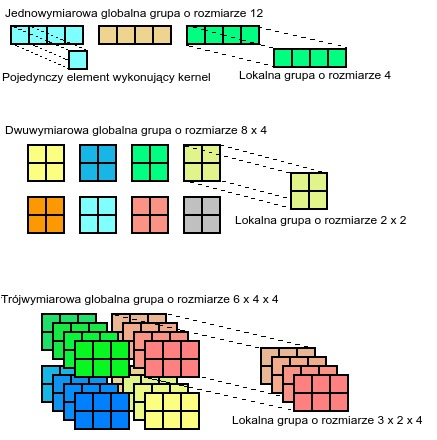
\includegraphics[scale=0.7]{imgs/KernelDispatch.jpg}
	\caption{N wymiarowy podział kernela}
\end{figure}
Na samym końcu zawołane zostaje \textbf{clFinish}. Jest to funkcja blokująca po wykonaniu, której mamy pewność, że wszystkie zakolejkowane na konkretnej kolejce operacje zostały wykonane.
W wyniku działania takiego kodu w buforze znajdować się będą 1024 elementy o wartości 13131314.
\subsection{Możliwości i ograniczenia sprzętowe}
Każde urządzenie posiada ograniczenia związane ze specyfiką implementacji sterownika oraz barkiem zasobów sprzętowych. By dowiedzieć się jakie są maksymalne dostępne wartości, np. dotyczące rozmiaru pamięci, ilości poszczególnych obiektów w kernelu czy maksymalnej liczbie dostępnych work itemów w ramach lokalnej work grupy, możemy odpytać sterownik wołając clGetDeviceInfo, podając konkretny parametr. Dzięki temu wykonywana aplikacja może dostosować się do ograniczeń sprzętowych. Oto wynik działania aplikacji "clinfo", która wypisuje wszystkie dostępne informacje o urządzeniu. W tym wypadku jest to telefon Xiaomi Mi a2 lite z procesorem graficznym Adreno 506.
 \lstinputlisting{listings/clinfo.log}
 \subsection{Pomiary czasu wykonywania kerneli}
 Standard OpenCL zapewnia mechanizm do odczytywania stempli czasu z poszczególnych etapów wykonywania kernela. Służy do tego obiekt typu cl\_event stworzony przez funkcje clCreateUserEvent. Obiekt taki może zostać przekazany jako argument funkcji, która zostanie wykonana na urządzeniu, np. clEnqueueNDRangeKerne czy clWnqueueWriteBuffer.
 Po wykonaniu kernela z obiektu eventa można odczytać stemple czasu z jego wykonania. By wydobyć wartości należy zawołać clGetEventProfilingInfo, przekazując jako argument obiekt eventu oraz jeden z czterech parametrów .
 \begin{itemize}
     \item CL\_PROFILING\_COMMAND\_QUEUED wartość opisuje czas urządzenia, w którym komenda została dodana do kolejki.
     \item CL\_PROFILING\_COMMAND\_SUBMIT wartość opisuje czas urządzenia z momentu wysłania komendy do urządzenia na którym zostanie wykonana.
     \item CL\_PROFILING\_COMMAND\_START wartość opisuje czas urządzenia, w którym rozpoczęte zostało wykonywanie komendy na urządzeniu.
     \item CL\_PROFILING\_COMMAND\_END wartość opisuje czas urządzenia, w którym wykonywanie komendy zostaje zakończone.
\end{itemize}
\subsection [Współdzielenie obiektów pomiędzy OpenCL i OpenGL]{Współdzielenie obiektów pomiędzy OpenCL i OpenGL}
OpenGL (z ang. Open Graphics Library) to standard, który tak jak OpenCL jest zdefiniowany i utrzymywany przez grupę Khronos. Jest on wykorzystywany głównie do renderowania obiektów graficznych.
Istnieje możliwość stworzenia textury w OpenGL i użycie jej w kernelu OpenCL. Nie wszystkie urządzenia wspierają współdzielenie zasobów. Jeśli w liście rozszerzeń znajduje się cl\_khr\_gl\_sharing, możliwe wtedy jest użycie z tego rozwiązania. Chcąc skorzystać tej możliwości, kontekst w OpenCL musi zostać stworzony w oparciu o wcześniej stworzony kontekst OpenGL. Przy tworzeniu kontekst podajemy strukturę, w której umieszczone są wskaźniki na kontekst w OpenGL i uchwyt na EGLDisplay. 
 \lstinputlisting{listings/contextProperties.txt}
 Posiadając tak stworzony kontekst, możemy stworzyć obiekt obrazka w OpenCL w oparciu o stworzoną teksture w OpenGL.
 \lstinputlisting{listings/sharedImage} W podanym wyżej kodzie, textureId to identyfikator tekstury, którą chcemy współdzielić z openGL. 
 Przed wykorzystaniem współdzielonego obrazka należy zawołać clEnqueueAcquireGLObjects, wskazując kolejkę, która będzie używać obrazka. Jest to wykonywane w celu wywłaszczenia obiektu przez OpenCL. Po zakończeniu operacji należy zwolnić obiekt poleceniem clEnqueueReleaseGLObjects.



